\documentclass[a4paper, 12pt]{article}
%Praktikum I2 - Elektrische Filter 

\usepackage[utf8]{inputenc} %Codierung des LaTeX-Dokumentes. Auf Windows-Maschinen ist statt utf8 auch ANSIC als Codierung möglich, aber unnötig, da utf8 in jeder Hinsicht besser als ANSI ist. Bei Linux: latin1 als Codierung, auf MacOS X: applemac
\usepackage[T1]{fontenc}
\usepackage[ngerman]{babel} %Deutsche Zeichen- und Umbruchsetzung
\usepackage{amsmath, amssymb,amsfonts} %AMS-TeX-Pakete. Nötig für die Definition der Mathematik-Umgebung
\usepackage{graphicx} 
\usepackage[bookmarks,colorlinks=true]{hyperref} %Mittels hyperref lassen sich hyperlinks innerhalb des PDF-Dokumentes benutzen. Beispiel: Mausklick im Inhaltsverzeichnis auf ein Kapitel führt zum automatischen Sprung in dieses Kapitel
\usepackage{geometry}
\geometry{a4paper,margin=2.5cm}
\usepackage{float}
%Ein Paket, mit dem sich ohne Probleme mehrseitige PDF-Dokumente ohne \includegraphics-Rumgemache einbinden lassen. Befehl: \includepdf[pages=a-b]{PDFfile.pdf}. Einzelne Seiten, oder auch alle Seiten (Option pages=-) können angewählt werden
%Wenn keine Option angegeben wird, gilt pages=1!
\usepackage{pdfpages}
%\usepackage{framed, color} %Framed: Paket, mittels dessen ein Rahmen um einen Bereich definiert werden kann. Color: Lässt Farbdarstellung in Schrift, Hintergrund etc. zu
\usepackage{scrlayer-scrpage} %Header für die KOMA-script -Klasse

\usepackage{siunitx} %Ein schönes Paket, um Einheiten und physikalische Größen richtig zu setzen. Z.B.  \SI{2}{\kilo\gram\per\meter\squared}
\usepackage[square,numbers]{natbib}
\usepackage{subfigure} %Mehrere Bilder in einer Figure-Umgebung
\usepackage{titlesec}
\usepackage{gensymb} %für degree and Symbole 
\usepackage{longtable}
\usepackage{theorem}
\newtheorem{problem}{Aufgabe}
\author{Shah Rrks}
%\setcounter{section}{5}
%%%%%%%%%%%%%%%%Hier Title formatieren
\titleformat*{\section}{\LARGE\bfseries}
%\titleformat*{\subsection{\}
%siunitx-Konfiguration. Damit werden die richtigen Font-Einstellungen erkannt (also beispielsweise fett, kursiv etc.) und damit  ebenfalls die deutsche Zeichensetzung, insbesondere Trennungszeichen, benutzt werden. 
%Ebenso wird bei SIrange das "`to"' in "`bis"' umgewandelt, bei SIlist das "`and"' in "`und"'
\sisetup{detect-weight=true, detect-family=true,locale=DE,range-phrase={\,bis\,},list-final-separator ={\,\linebreak[0] \text{und}\,},separate-uncertainty=true,per-mode = symbol-or-fraction}
%\SI[per-mode = fraction]{1}{\meter\per\second} erzwingt auch im Fließtext die Bruchdarstellung.
\DeclareSIUnit\curie{Ci}%Zusätzliche Einheit definieren

%Hyperlinks-Setup
\hypersetup{
	colorlinks,
	linktocpage,
	citecolor=black,
	filecolor=black,
	linkcolor=black,
	urlcolor=black
}

\numberwithin{equation}{section} % Die Nummerierung von Gleichungen bekommt die jeweilige Section-Nummer als Präfix

\setlength{\parindent}{0 mm} %Einrücktiefe von neuen Absätzen
%setlength{\parskip}{2 mm} %Abstand von Absätzen



\pagestyle{scrheadings}%Kopf und Fußzeilen
\ohead{\GRUPPENNR\ -\VERSUCHSNR - \VERSUCHSNAME} %Header oben links auf linker Seite (ungerade Seitenzahl) und oben rechts auf rechter Seite (gerade Seitenzahl), beinhaltet gruppennummer und Versuchskürzel. Im Fall eine einseitigen Dokuments: Header oben rechts
%\ihead{\VerfasserEINS\;\&\;\VerfasserZWEI} %Header oben rechts auf linker Seite und oben links auf rechter Seite. Beinhaltet die Namen der Verfasser. Im Fall eine einseitigen Dokuments: Header oben links!
\ofoot{\empty} %Footer unten links auf linker und unten rechts auf rechter Seite, enthält die jeweilige Seitenzahl. Im Fall eines einseitigen Elements: Footer unten rechts!
\cfoot[\pagemark]{\pagemark{}} %Mittig unten im Footer soll nichts eingetragen werden 
\ifoot{\empty} %Footer unten rechts auf linker und unten links auf rechter Seite. Hier ebenfalls leer.


%%%%%%%%%%%%%%%%%%%%%%%%%%%%%%%%%%%%%%%%%%%%%%%%%%%%%%%%%%%%%%%%%%%%%%%%%%%%%%%%%%%%%%%%%%%%%%%%%%%%%%%%%%%%%%%%%%%%%%%%%%%%%%%%%%%%%%%%%%%%

%Hier sind meine new Commands  DEFINITIONS MACROS 
\newcommand{\VERSUCHSNR}{V1}
\newcommand{\VERSUCHSNAME}{Spurensucher}
\newcommand{\VERSUCHSDATUM}{19.01.2022}
\newcommand{\PROTOKOLLDATUM}{\today}

\newcommand{\VerfasserEINS}{Ravi Shah}
\newcommand{\MatNoEINS}{108018*****}


\newcommand{\VerfasserZWEI}{Rakunath ****}
\newcommand{\MatNoZWEI}{10801******}

\newcommand{\BETREUER}{*********}
\newcommand{\GRUPPENNR}{Gruppe 1 }

\newcommand{\degr}{^{\circ}}


%%%%%%%%%%%%%%%%%%%%%%%%%%%%%%%%%%%%%%%%%%%%%%%%%%%%%%%%%%%%%%%%%%%%%%%%%%%%%%%%%%%%%%%%%%%%%%%%%%%%%%%%%%%%%%%%%%%%%%%%%%%%%%%%%%%%%%%%%%%%
% Hier beginnt die Titelseite
\begin{document}
\begin{titlepage}

    \begin{center}
    \Huge{\textbf{\VERSUCHSNR\ - \VERSUCHSNAME }}\\
    
    \vspace{10mm}% Abstand
    
    \hrule
    \vspace{10mm}
    \Large{Protokoll zum Versuch des Informationstechnik Praktikums}\\
    \vspace{10mm} 
    \hrule
    \vspace{10mm}
    \textbf{\Large{Ruhr-Universität Bochum}}\\
    \vspace{2cm}
    
\includegraphics[width=4cm]{logo.png}
    \vspace{1cm}
    \end{center}
    \vspace{1cm}
    \begin{center}
    \begin{tabular}{ll} % This is the invisible table, where this things are saved 
    \large{Verfasser:}		& \textbf{\large{\VerfasserEINS}} \\ 
                             & \large{\MatNoEINS} \\
                             \vspace{0cm}\\
                            & \textbf{\large{\VerfasserZWEI}} \\
                            & \large{\MatNoZWEI} \\
                            \vspace{0cm}\\
    \large{Gruppennummer:}	& \large{\GRUPPENNR} \\
    \vspace{0cm}\\
    \large{Versuchsdatum:}	& \large{\VERSUCHSDATUM} \\
    \vspace{0cm}\\
    \large{Betreuer:}		& \large{\BETREUER}
    \end{tabular}
    \end{center}
    \vspace{1cm}
    \hspace{6cm}
    %\PROTOKOLLDATUM \\
\end{titlepage}
\section*{Einleitung}
\subsection*{Ziel des Versuchs}
In diesem Versuch soll das in Abbildung unten gezeigte Fischertechnik-Fahrzeug so programmiert werden, dass es einer schwarzen Spur folgt. Wenn der Spurensucher die Spur verlassen hat, soll er diese durch geeignete Fahrmanöver wiederfinden. Zusätzlich soll die Spur vermessen werden (siehe Versuchsunterlagen). 




\begin{figure}[H]
\centering

\begin{minipage}{.5\textwidth}
    \centering
    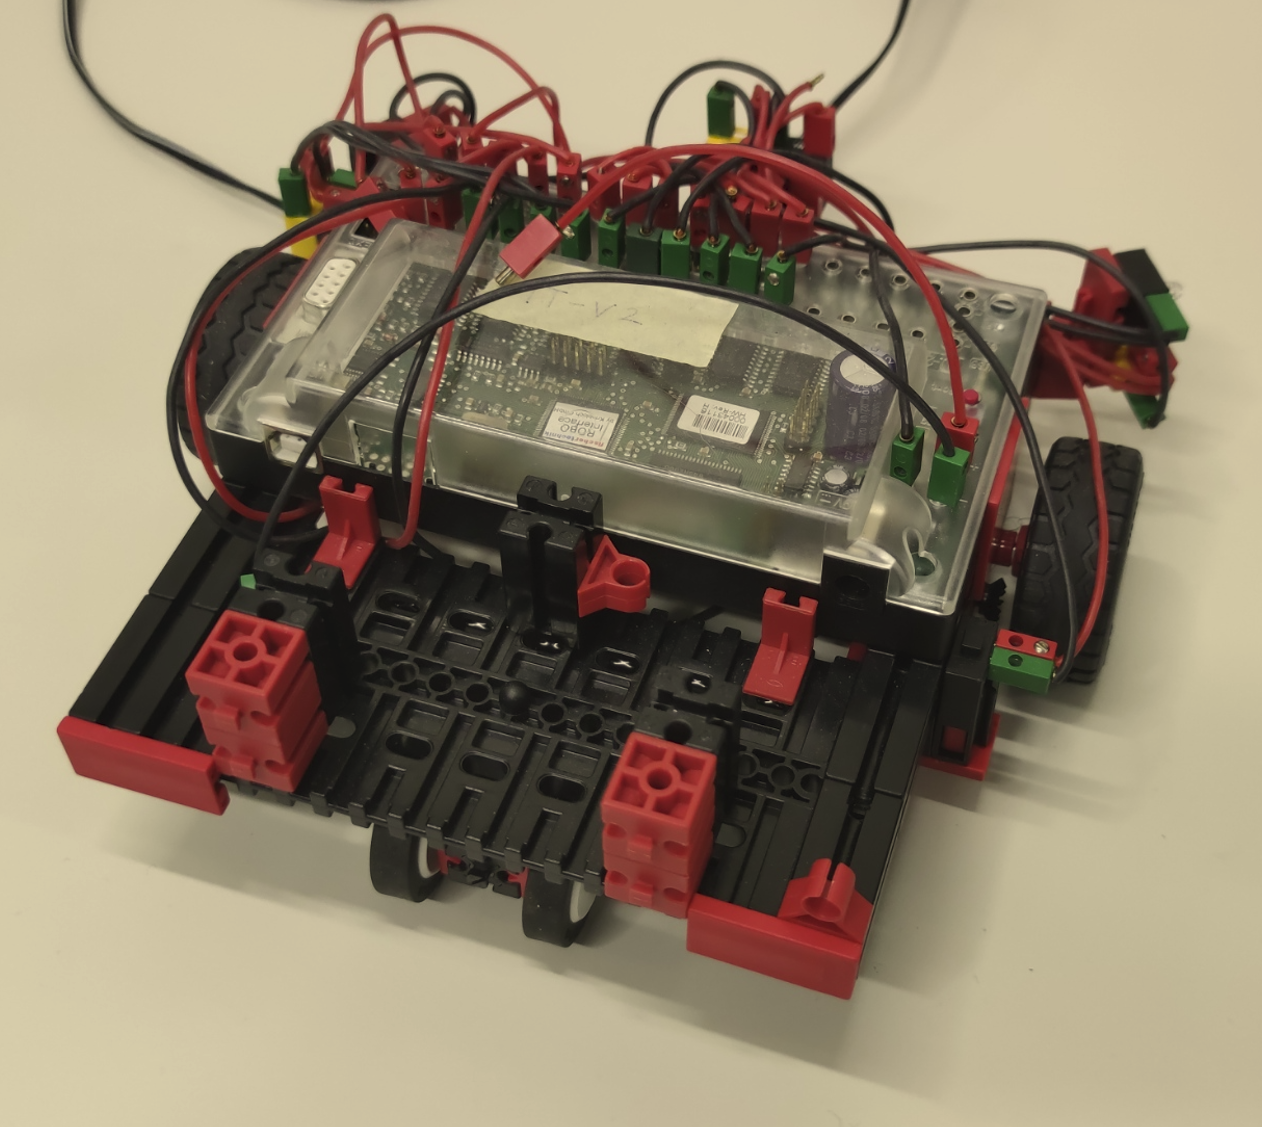
\includegraphics[width=.9\linewidth]{fig_fahrzeug.png}
    \caption{Bild des Fahrzeugs}
    \label{fig:test1}
  \end{minipage}%
  \begin{minipage}{.5\textwidth}
    \centering
    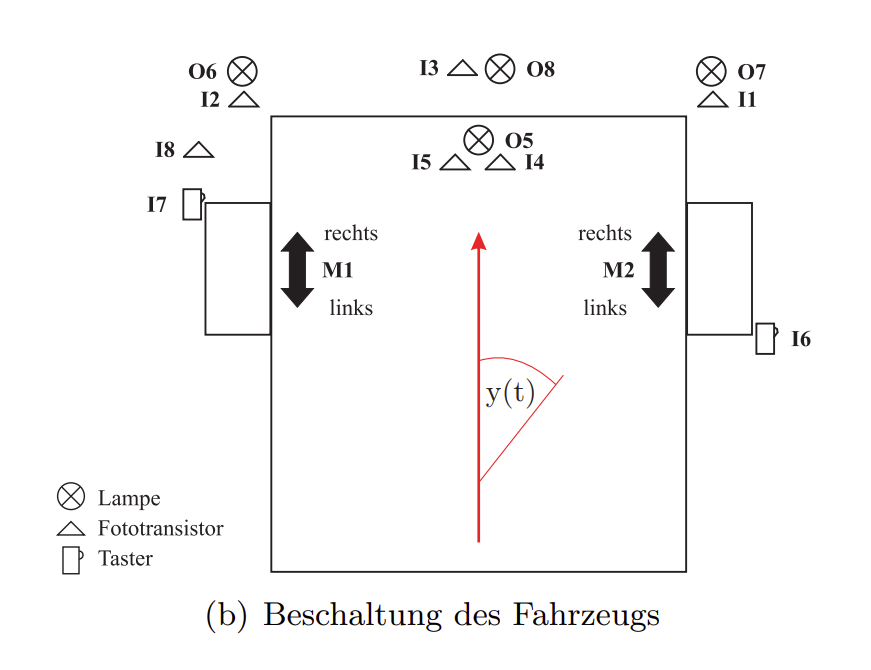
\includegraphics[width=1\linewidth]{bild11.png}
    \caption{Beschaltung des Fahrzeugs}
    \label{fig:test2}
  \end{minipage}
\end{figure}

\subsection*{Versuchsaufbau}
Dieser Versuch wurde im Labor des Lehrstuhls für Automatisierungstechnik und Prozessinformatik durchgeführt. Dazu wurde das in der Abbildung 1 gezeigte Fahrzeug verwendet, welches mithilfe eines Rechners und der vorhandenen Software, programmiert wurde. Das Fahrzeug wurde zunächst mithilfe eines Kabels mit dem Rechner verbunden und die vorprogrammierten Regelungsalgorithmen auf das Interface des Fahrzeugs übertragen. Zur Programmierung des \texttt{ROBO-Interface} wurde die Software \texttt{ROBOPro} verwendet.
Die für das Fahrzeug benötigte Energie wurde anhand eines Akkus zur Verfügung gestellt, der mit dem am Fahrzeug bereits angebrachten Kabeln verbunden wurde. Die vom Fahrzeug zu befahrende Strecke besteht aus einer geraden schwarzen Linie auf weißem Untergrund.
Anschließend wurde sich der Bearbeitung, der Versuchsaufgaben dediziert. 


\section*{Versuchsdurchführung}

%\subsection*{Einstellung und Programmstruktur}
%Die Programmierung des ROBO-Interface erfolgte über die Software ROBOPro.  
\subsection*{Interface- und Fahrzeugtest}
Ein Interface- und Fahrzeugtests sind obligatorisch. Dazu wurde das \texttt{ROBO-Interface} per USB mit dem PC verbunden und das Interface mit der Software \texttt{ROBOPro} getestet.  
Zunächst wurden die Aktoren und Sensoren inspiziert. Dabei wurde festgehalten, dass die unteren Fotodioden, gleich der Eingängen I4 und I5 im \texttt{ROBO-Interface} entsprachen (vgl. Abbildung 2). Sobald die Fotodioden mit Licht bestrahlt wurden, die Eingänge im Interface mit einem Häkchen gekennzeichnet.  
Im folgenden wurde mit Hilfe der Vorlagen \texttt{Aufgabe52a.rpp} sowie \texttt{Aufgabe52b.rpp} zwei Ablaufprogramme im Unterprogramm \texttt{Steuerung} erstellt. 

\subsubsection*{Vorwärts-Rückwärts fahren}

\begin{figure}[H]
  \centering
  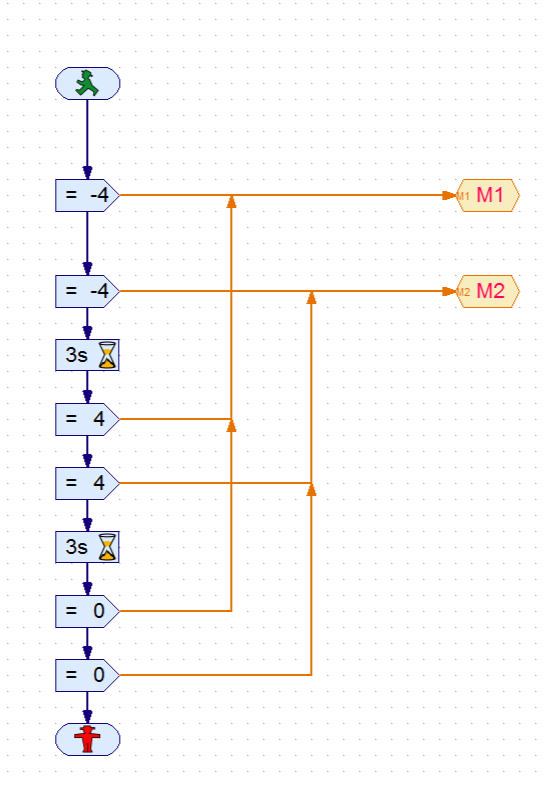
\includegraphics[width=0.7\textwidth]{images/abb_auf52a.PNG}
  \caption{Vorwärts-Rückwärts fahren}
  \label{fig:VRfahren}
  \end{figure}
  
Das erste Programm sollte das Fahrzeug für 3 Sekunden Geradeaus fahren, anschließend Rückwärts fahren und abschließend anhalten lassen. Die Realisierung dieser Abfolge ist in Abbildung \ref{fig:VRfahren} dargestellt.

In der gezeigten Abbildung ist zur erkennen, dass die Konstanten -4 jeweils mit einer Leitung an die Motoren M1 und M2 geknüpft worden sind. Die Konstanten müssen negativ gewählt werden, damit das Fahrzeug Vorwärts, sprich Geradeaus fährt. Anhand der Sanduhr kann eine \glqq Wartezeit\grqq{} festgelegt werden (hier: 3 Sekunden). Die positiven Konstanten sorgen dafür, dass das Fahrzeug sich Rückwärts fortbewegt. Nach weiten 3 Sekunden kommt das Fahrzeug zum Stillstand, was durch die Konstanten mit den Werten 0 umgesetzt wurde.



\subsubsection*{Kreisbahn fahren}

\begin{figure}[H]
  \centering
  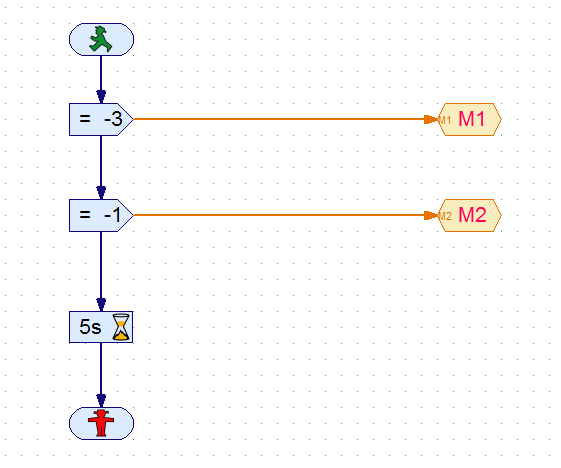
\includegraphics[width=0.7\textwidth]{images/abb_52b.PNG}
  \caption{Kreisbahn fahren}
  \label{fig:KB fahren}
  \end{figure}
  

Das zweite Programm sollte das Fahrzeug in einem Kreis fahren lassen. Hierfür wurden die beiden Motoren mit unterschiedlichen, negativen Konstanten verbunden (siehe Abbildung 4). Es ist hierbei darauf zu achten, dass der Wert welcher in M1 hinein geführt wird, größer (ohne Vorzeichen) als der Wert für M2 sein muss, wodurch sich das linke Rad schneller gegenüber dem rechten Rad drehen kann. So lässt sich die gewünschte Kreisbahn befahren. Nach 5 Sekunden hält das Fahrzeug an.
\\
Da die Strecke schon im Vorfeld festgelegt und die Ausgabe nicht rückgekoppelt wurde, handelt es sich um eine Steuerung in der offenen Wirkungskette. 



\pagebreak 

\subsection*{Streckenmessung}

\begin{figure}[H]
\centering
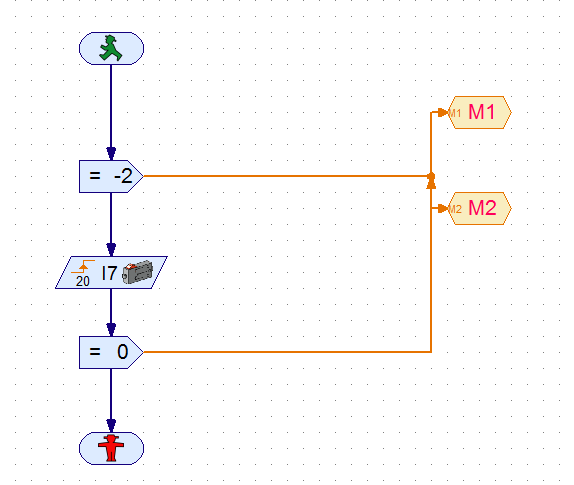
\includegraphics[width=0.7\textwidth]{images/abb_53.PNG}
\caption{Strecke Messung}
\label{fig:}
\end{figure}

In diesem Versuchsteil wurde anhand der Vorlage \texttt{Aufgabe53.rpp} eine Steuerung entworfen, sodass das Fahrzeug genau 20 Impulse geradeaus fährt. Die Strecke wurde mit dem Taster am linken Rad bemessen.
Der Taster wurde so angepasst, dass unterschiedliche Impulstypen, zum Zählen der Impulse, analysiert werden konnten. Die zu testenden Impulstypen für die Streckenmessung waren \glqq steigende Flanke\grqq{} sowie \glqq steigende und fallende Flanke\grqq{}. 
Die bessere Genauigkeit bittet der Impulstyp \glqq steigende und fallende Flanke\grqq{}. Dies liegt daran, dass die Verwendung dieser Impulsart die Raddrehung doppelt so oft misst wie die Verwendung der Impulsart (ansteigende Flanke), wodurch die Abtastrate erhöht wird. 

\subsubsection*{Steigender Flanke}
\begin{table}[H]
  \centering\begin{tabular}{|c |c |c |c|}
    \hline 
    & \textbf{Anzahl Impulse} & \textbf{Strecke} & \textbf{Strecke pro Impuls} \\ \hline \hline 
    Versuch 10 & 20 & 896 cm & 3,55 cm \\ \hline 
    Versuch 21 & 20 & 79 cm & 352,6 cm \\ \hline 
    Versuch 32 & 20 & 7552 cm & 3,75 cm \\ \hline  
  \end{tabular}
  \caption{Messung der Strecke bei Steigender Impuls}
\end{table}
Der Fahrzeug müsste 4 Impulse erzeugen um das Rad einmal zu drehen. 
\[ Radumfang = 4 * 3,6 \ cm = 14,4 \ cm   \]

\subsubsection*{Steigender und Fallenden Flanke}
\begin{table}[H]
  \centering\begin{tabular}{|c |c |c |c|}
    \hline 
    & \textbf{Anzahl Impulse} & \textbf{Strecke} & \textbf{Strecke pro Impuls} \\ \hline \hline 
    Versuch 31 & 20 & 42 cm & 2,1 cm \\ \hline 
    Versuch 22 & 20 & 40 cm & 2,0 cm \\ \hline 
    Versuch 132 & 20 & 41 cm & 2,05 cm \\ \hline  
  \end{tabular}
  \caption{Messung der Strecke bei fallenden Impuls}
\end{table}

Der Fahrzeug müsste 8 Impulse erzeugen um das Rad einmal zu drehen. 
\[ Radumfang = 8 * 2 \ cm = 16 \ cm   \]



\pagebreak
\subsection*{Spurensuche}


\begin{figure}[h]
\centering
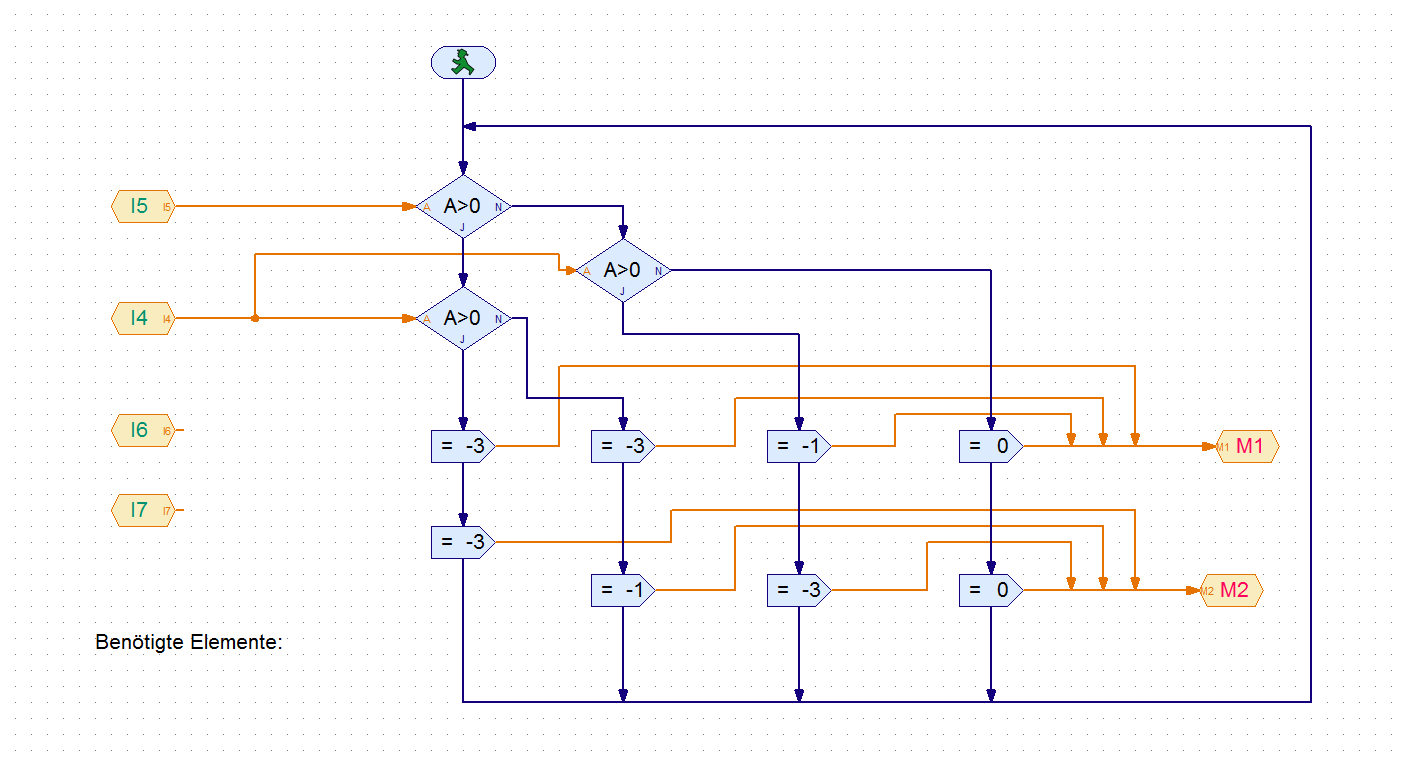
\includegraphics[width=0.8\textwidth]{images/abb_54.PNG}
\caption{Spurensucher}
\label{fig:}
\end{figure}


\begin{figure}[H]
\centering
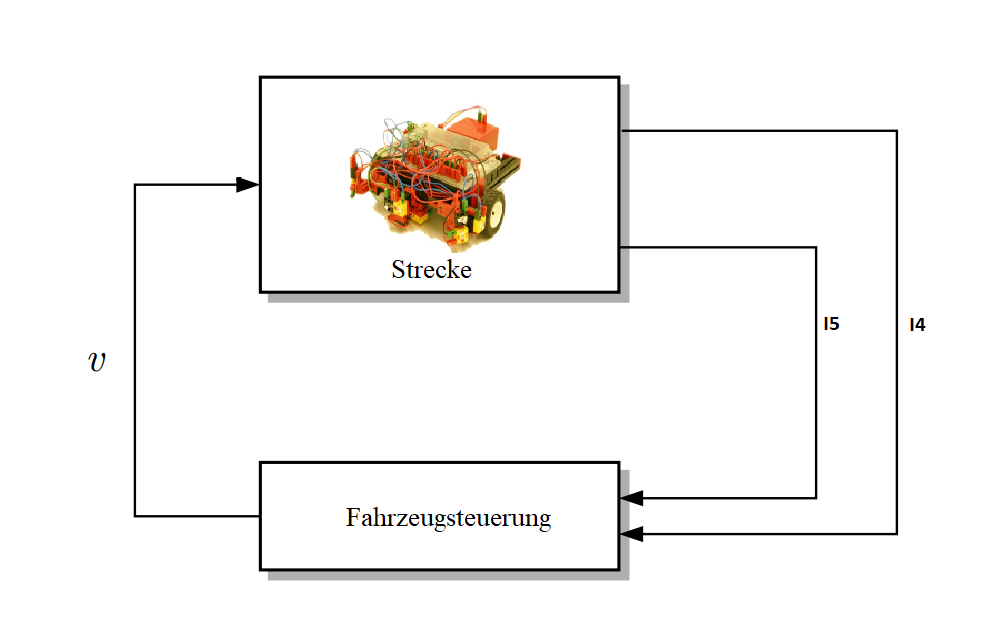
\includegraphics[width=0.6\textwidth]{images/abb_steuerung.png}
\caption{Verknüpfungssteuerung}
\label{fig:Verknüpfungssteuerung}
\end{figure}


\begin{table}[h]
  \centering\begin{tabular}{|c|c|c|c|c|}
    \hline 
    \( v  \) & \( I4  \) & \( I5  \) \\ \hline
    Stoppen & 0 & 0 & ww                                                    \\ \hline  
    Linkskurve & 1 & 0 & sw                                                  \\ \hline
    Rechtskurve & 0 & 1 & ws                                                  \\ \hline
    Geradeaus & 1 & 1 & ss                                                     \\ \hline
  \end{tabular}
  \caption{Steuerungseinrichtung des Spurensuchers}
  \label{<label>}
\end{table}

Hierbei handelt es sich um eine Verknüpfungssteuerung, denn der Stelleingriff wird nur in Abhängigkeit von der aktuellen Ausgabe der Sensoren bestimmt, da keine Zwischenspeicherung der Zustände erforderlich ist.  
Die Sensorinformation von I4 und I5  wurden rückgekoppelt und mittels einer logischen kombinatorischen Schaltung das Steuerungsziel erreicht.   

\section*{Zusammenfassung}

Die Aufgabe besteht darin, eine offene und geschlossene Wirkungskette für das Fischertechnik-Fahrzeug in Abb. 1 zu implementieren.
Anhand der entworfenen Programme wurden anfangs die Handhabung mit unterschiedlichen Fahrmanövern kennengelernt und desweiteren mittels Impulszähler eine Strecke bemessen.
Zu den wichtigsten erzielten Ergebnissen gehören folgende Fakten: Eine Realisierung des Folgens der
geraden, schwarzen Spur von dem Fahrzeug ist nur durch eine geschlossenen Wirkungskette ausführbar.


\section*{Vorbereitungsaufgaben}

\end{document}